\section{Experimental results}
In this section we present experimental results for the simplicial neural network. The datasets we analyze have been extracted from the Semantic Scholar datasets. The data consists of XXX papers together with their authors and number of citations. We retain paper with more than $5$ citations and at most $10$ authors.

An important step in preprocessing many kinds of input data in TDA is constructing a simplicial complex. Our work focus on \emph{collaboration complexes} (or \emph{co-authorship complexes}) \stefania{cite paper Alice}, simplicial complexes where a paper with $k$ authors is represented by a $(k-1)$-simplex. We constructed different co-authorship complexes by considering sub-samplings from the papers set of the Semantic Scholar dataset. The sub-samplings were obtained by performing random walks on the nodes of the graph which vertices corresponds to the papers and edges connect papers sharing at least one author. The co-authorship complexes obtained from each sub-sampling  have corresponding $k$ co-chain given by the number of shared citations.

We evaluate the performance of the SNN on the task of predicting missed input data. 
Specifically, given a fixed co-authorship complex missing data is introduced 
at random on the training co-chains at $4$ levels: $10\%,  20\%,  30\%$, and $50\% $.  We trained a SNN composed by $3$-layers with $30$ convolutional filters. \stefania{Say how laplacian is build and size input} The training input is given by the citations on the co-authorship complex where the random missing data is substituted by the median of the known data. We used the $L_1$ norm as reconstruction loss over the known elements an the Adam optimizer with learning rate of $1\times 10^{-3}$. \stefania{Clarify what is test and train} Our evaluation  focus on the accuracy of the network in predicting the missing data. A predicted citation is considered correct if the predicted value differs of at most $1$ from the actual number of citations.

Figure~\ref{fig:accuracy} shows the accuracy results of the prediction of the missing citations on CC1 (Co-authorship Complex 1). The number of simplices per dimension in CC1 can be seen in Table~\ref{table:Simplices-coauthor}
\begin{table}
  \caption{%
  Number of simplices
  }
  \label{Simplices-coauthor}
  \centering
  \begin{tabular}{llllllllllll}
    \cmidrule(r){1-12}
    Dimension   & 0     & 1  & 2     & 3 & 4     & 5 & 6    & 7 & 8   & 9 & 10\\
    \midrule
    CC1 & 352  & 1474  & 3285  & 5019  & 5559  & 4547  & 2732  & 1175  & 343 & 61 & 5\\
    CC2 & 333 & 4444 & 333 & 4444 & 333 & 4444  & 333 & 4444  & 333 & 4444 &3333\\ 
    \bottomrule
  \end{tabular}
\end{table}
%\begin{figure}[htbp]
%  \centering
 
%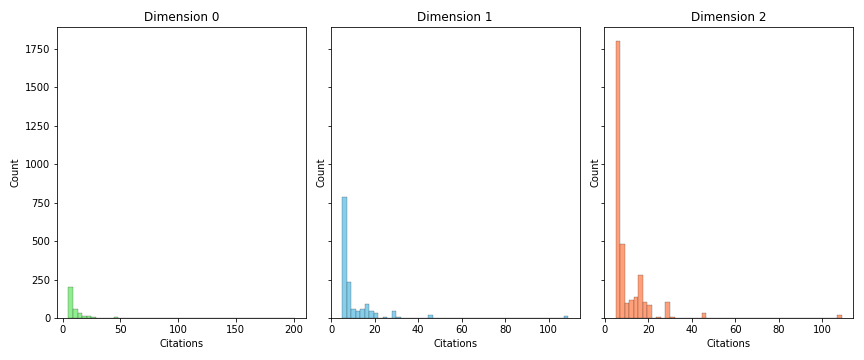
\includegraphics[scale=0.35]{./figures/distribution_cohain_150250.png}
% \caption{Distribution of the citation in CC1 } \label{fig:accuracy}
%\end{figure}
\begin{figure}[htbp]
  \centering 
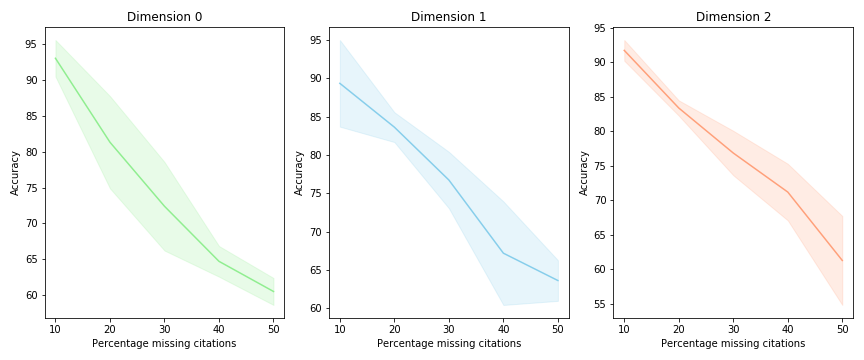
\includegraphics[scale=0.38]{./figures/accuracy_network1.png}
 \caption{Accuracy of SNN in predicting missing citations } \label{fig:accuracy}
\end{figure}

As a second assessment we evaluate how accurately a SNN pretrained on a co-authorship complex can predict citations on a different complex. The SNN with the same characteristic as above was trained on CC2 (Co-authorship Complex 2)


\stefania{Write number of iterations!}


\begin{figure}[htbp]
  \centering
 
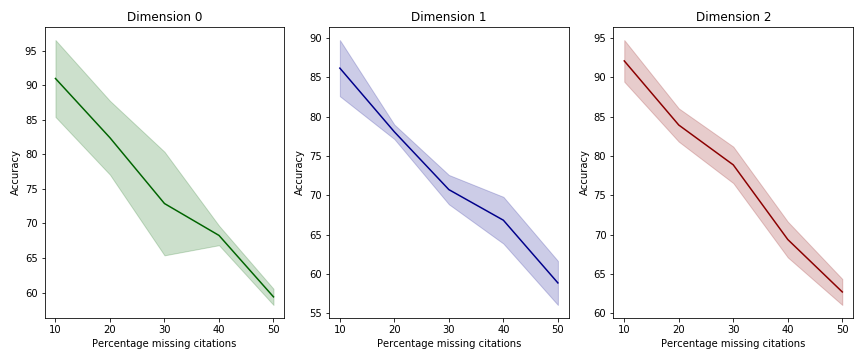
\includegraphics[scale=0.38]{./figures/accuracy_network1_pretrained.png}
  \caption{Accuracy in predicting missing citations with a pretrained SNN \stefania{Transfer learning?}} \label{fig:accuracy-pretrained}
\end{figure}

\begin{figure}[htbp]

  \centering
 \hspace{-6cm}
 
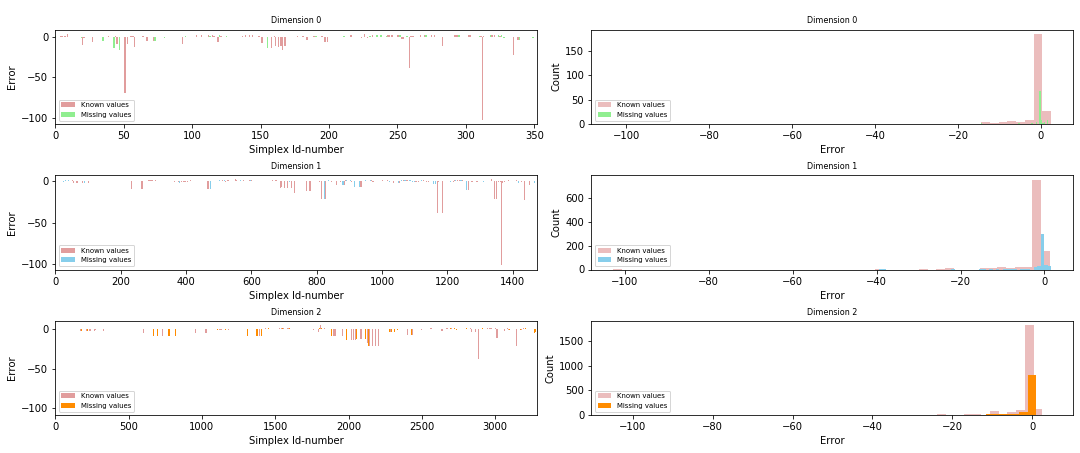
\includegraphics[scale=0.4]{./figures/Error_start150250_seed6666_notsee30.png}
  \caption{Distribution of the prediction's error} \label{fig:error}
\end{figure}

\stefania{PLot only error distribution in log-scale}